\subsection{Cambio dataset caricato}

\begin{figure}[H]
    \centering
    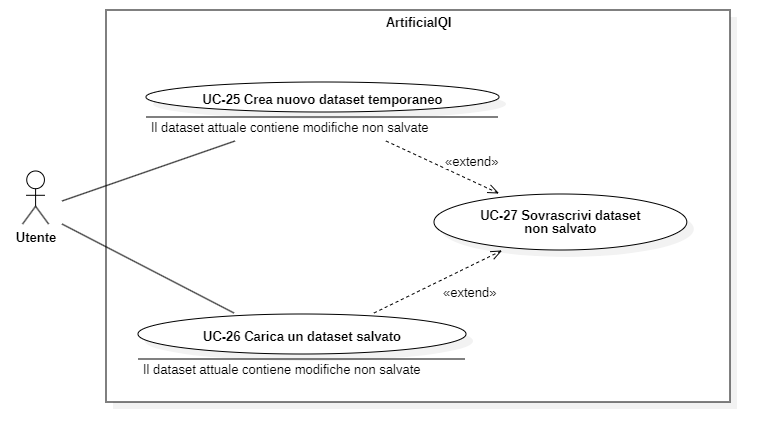
\includegraphics[scale=0.53]{Sezioni/UseCase/Immagini/CambioDatasetCaricato.png}
    \caption{Diagramma cambio dataset caricato.}
\end{figure}

\begin{usecase}{UC-25}{Crea nuovo dataset temporaneo}
    \label{uc:UC-25}
    
    \req{\hyperref[ru:RUO-3]{RUO-3}} 

    \pre{
        \item L'utente sta visualizzando la lista dei dataset salvati
    }

    \post{
        \item Il sistema carica un nuovo dataset vuoto
    }
    
    \actor{Utente}

    \subactors{}

    \trigger{L'utente vuole creare un nuovo dataset temporaneo}

    \inc{}

    \base{}

    \scenario{
        \item L'utente richiede la creazione di un nuovo dataset
        \item Il sistema verifica che il dataset attualmente caricato non abbia modifiche non salvate
        \item Il sistema carica un nuovo dataset vuoto temporaneo
    }

    \subscenario{
        \item[2.1] Il dataset caricato contiene modifiche non salvate:
        \begin{itemize}
            \item \hyperref[uc:UC-27]{UC-27}
        \end{itemize}
    }
\end{usecase}

\begin{usecase}{UC-26}{Carica un dataset salvato}
    \label{uc:UC-26}
    
    \req{\hyperref[ru:RUO-6]{RUO-6}} 

    \pre{
        \item L'utente sta visualizzando la lista dei dataset salvati
    }

    \post{
        \item Viene caricato il dataset salvato indicato
    }
    
    \actor{Utente}

    \subactors{}

    \trigger{L'utente richiede il caricamento di un dataset salvato}

    \inc{}

    \base{}

    \scenario{
        \item L'utente richiede il caricamento di un dataset salvato
        \item Il sistema verifica che il dataset attualmente caricato non abbia modifiche non salvate
        \item Il sistema carica il dataset salvato indicato
    }

    \subscenario{
        \item[2.1] Il dataset caricato contiene modifiche non salvate:
        \begin{itemize}
            \item \hyperref[uc:UC-27]{UC-27}
        \end{itemize}
    }
\end{usecase}

\begin{usecase}{UC-27}{Sovrascrivi dataset non salvato}
    \label{uc:UC-27}
    
    \req{} 

    \pre{
        \item Esiste un dataset con modifiche non salvate
    }

    \post{
        \item Il dataset attuale viene sovrascritto dal dataset caricato e le modifiche non salvate vengono perse
    }
    
    \actor{Utente}

    \subactors{}

    \trigger{Il dataset attuale contiene delle modifiche non salvate e il sistema deve caricarne un altro}

    \inc{}

    \base{}

    \scenario{
        \item L'utente richiede di sostituire il dataset attuale che presenta modifiche non salvate
        \item Il sistema richiede all'utente la conferma della sovrascrittura
        \item L'utente conferma la sovrascrittura
        \item Il sistema sovrascrive il dataset attuale con il dataset caricato e le modifiche non salvate vengono perse
    }

    \subscenario{
        \item[2.1] L'utente annulla la sovrascrittura:
        \begin{itemize}
            \item Il sistema interrompe l'operazione di caricamento
            \item Il dataset attuale resta invariato
        \end{itemize}
    }
\end{usecase}
